\chapter{Fundamentals}

This chapter presents the core concepts what are necessary that will support the next chapters. First, Hart's classical NILM technique is going to be described. Next, an introduction to mathematical optimization is presented. Finally, the NILM technique formulated as an optimization problem is presented. 

\section{NILM as a Pattern Recognition Problem}
This section is going to describe Hart's pattern recognition method which will be used to compare with the proposed method in the results section. The technique is fundamentally based on event detection and classification of pair of events with opposite direction. The major attention in this section to the characteristics of the algorithm. For further details, the reader may refer to \cite{hart} and \cite{hart85}. 

Fundamentally, Hart's method is based on the detection of steps in power measurements, as illustrated in the Figure \ref{illustration_ch2}. The algorithm is suitable for both a supervised or unsupervised approach. For each event, it is measured the available appliance signatures from the meter such as active power, reactive power, harmonics and duration. Those events might change depending on the information available in the smart meter. For example, smart meters with low sampling rate (which is the most common case), allows for limited signature information such as only the active power. The core of Hart's algorithm is illustrated in the Figure \ref{algorithm_ch2}. More details on each item of the figure are going to be discussed in the following items:

\begin{figure}[htb]
    \centering
    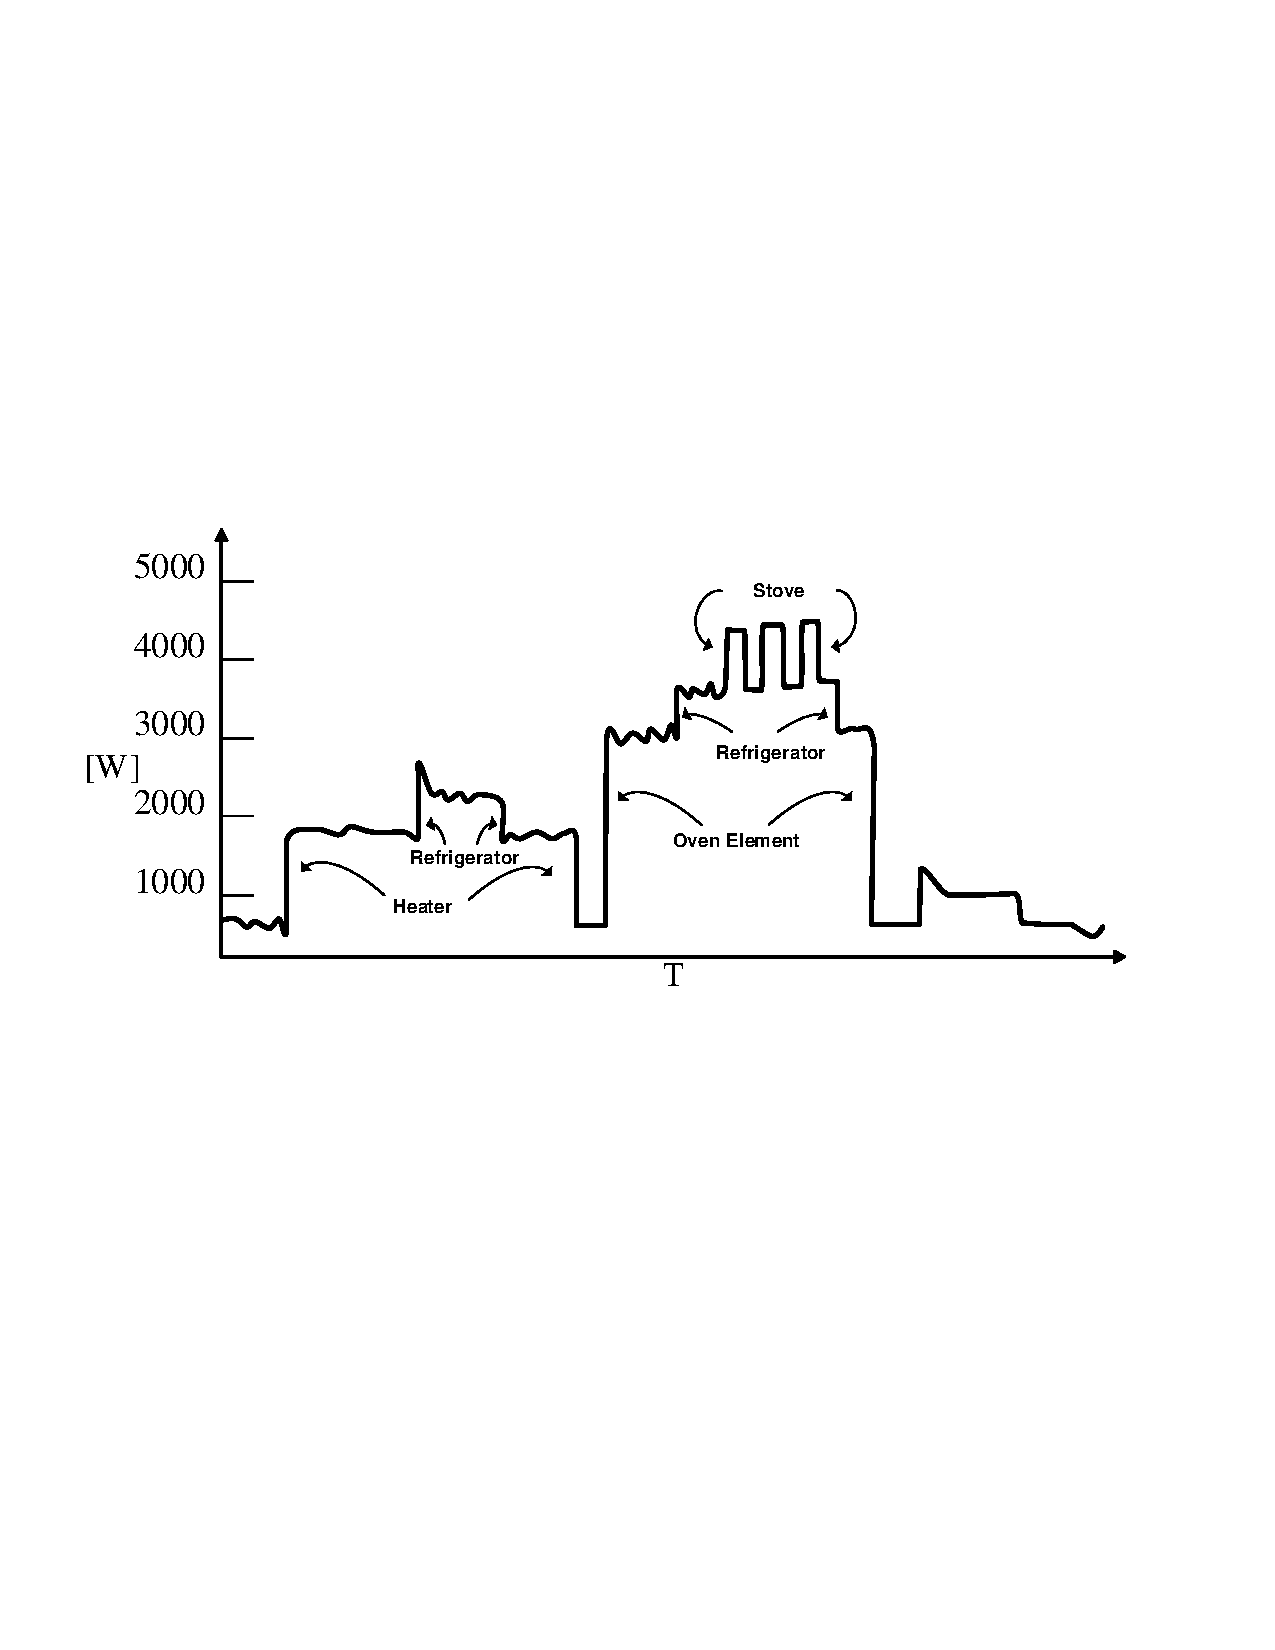
\includegraphics[width=1\columnwidth ]{illustration_ch2.pdf}
    \caption{Illustration of edges that could be detected from a typical power measurement.}
    \label{illustration_ch2}
\end{figure}



\begin{figure}[htb]
    \centering
    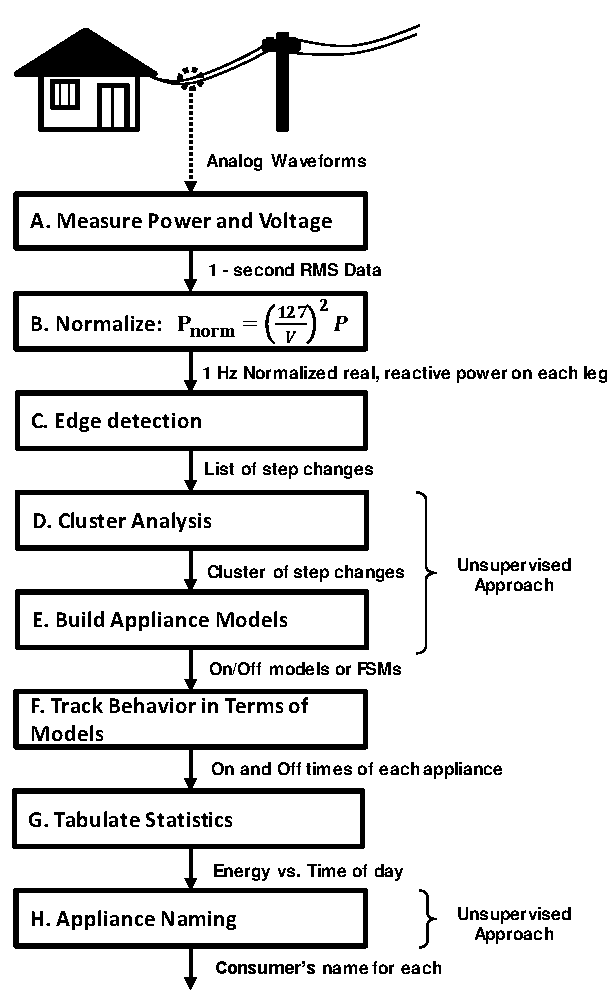
\includegraphics[width=0.5\columnwidth]{algorithm_ch2.pdf}
    \caption{Core steps of Hart's algorithm \cite{hart}.}
    \label{algorithm_ch2}
\end{figure}

\begin{itemize} 
    \item \textbf{Measure Power and Voltage:} Power and RMS voltage are averaged over intevals of one second. Voltage, real power and reactive power are digitally acquired based on a high sampling rate. 
    
    \item \textbf{Normalize Power:} The Equation \eqref{normalize} is used in order to compute the normalized total load power. The normalization translates into what the power would be if the utility provided a steady voltage and the load obeyed a linear model. 
    
    \begin{equation} \label{normalize}
         P_{norm}(t) = \frac{127}{V(t)}^2 P(t) 
    \end{equation}
    
    
    \item \textbf{Edge Detection:} The sizes of steplike changes and their times of occurrence (time stamp) are obtained by an edge detection algorithm. Hart defines two types of periods: steady period and periods of change. Steady period are defined as periods where the input does not change more than a threshold during a certain number of samples. Any other period that does not meet this criteria is defined as periods of change. The step size is calculated as the average of a steady period. The time stamp is provided by the time of the first sample in a changing period. The edge detection process is illustrated in the Figure \ref{edge_dect_ch2}.
    
        
\begin{figure}[htb]
    \centering
    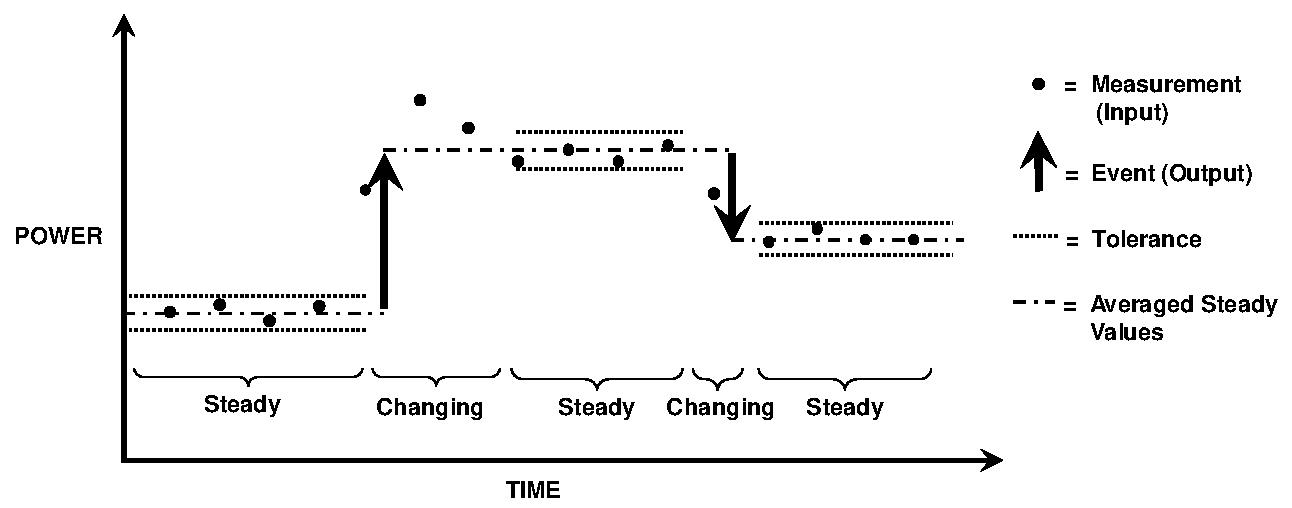
\includegraphics[width=1\columnwidth]{edge_dect_ch2.pdf}
    \caption{Illustration of the edge detection process of Hart's method \cite{hart}.}
    \label{edge_dect_ch2}
\end{figure}
    
    
    
    \item \textbf{Cluster Analysis:} The previously identified events are grouped into clusters. Each clusters is a set of events which are all close to each other. The Figure \ref{cluster_ch2} illustrates some clusters that might appear after the edge detection process. This task might get very difficult if many clusters of different appliances are intersecting each other. 
    
    \item \textbf{Appliance Models:} Models of appliances with simple ON/OFF states or multiple states are constructed. For ON/OFF appliances, the model is constructed by taking the centroid of symmetrical positive and negative clusters. In other words, pair of similar clusters representing positive and negative edges. The pair of centroids is matched involving a tolerance criteria. Models of appliances with multiple states are constructed by combining sequences of signatures. 

    \item \textbf{Track Behavior:} The available appliance models are tracked using a decoding approach. The approach is analog to a communication model where each appliance is considered a transmitter broadcasting their electrical measurements as information. The house wiring is the communication channel and finally the algorithm is the receiver. The decoding algorithm is based on a generalization of the Viterbi algorithm.\footnote{Optimal decoding technique based on dynamic programming} Giving a message source, the algorithm corrects errors that may occur in the channel such as insertions, deletions and merges. The details of the algorithm are presented in \cite{hart93}.  
    
    \item \textbf{Tabulate Statistics:} Energy statistics can be computed from the power levels and time stamp obtained in the previous step. Some example of useful statistics are the operating power, total energy and energy broken down by hour/day/week. The energy statistic is also useful for a conflict resolution step to check if there are more appliances activated than it should. It could be checked if the energy inferred from all appliances is higher than the total house power. This situation is likely to happen in cases where both OFF and immediately following ON event of an appliance are missed.   
    
    \item \textbf{Appliance Naming:} Finally, a name should be assigned to each appliance model detected from the collected data. Statistics based on the typical duration of an appliance can be useful for this task. Another useful information is the operating power level (127V vs 220V) of the device which is useful to check if the appliance is a single phase or two phase element. 

\end{itemize}



\section{Mathematical Optimization}
Mathematical optimization (also known as mathematical programming) is the process of minimization or maximization of an objective function of many variables, subject to constraints on the variables \cite{ampl}. The equation \eqref{opt_example} shows an example of optimization problem.

\begin{equation} \label{opt_example}
    \max_{x_i} \quad \sum_{i\ = 1}^{n} v_i\ x_i
\end{equation}

subject to 

\begin{equation}
    \sum_{i\ = 1}^{n} w_i\ x_i \ \leq \ W \quad \forall \ x \in \{0,1\}
\end{equation}

\begin{figure}[htb]
    \centering
    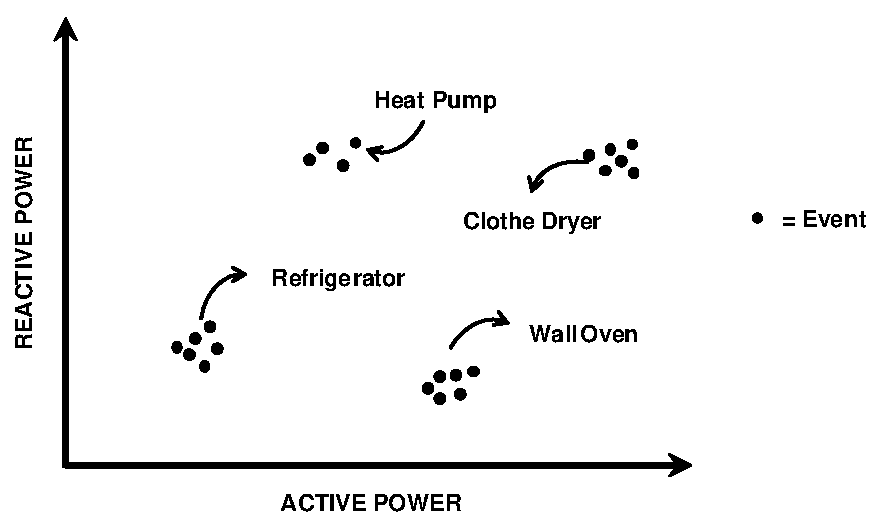
\includegraphics[width=1\columnwidth]{cluster_ch2.pdf}
    \caption{Hypothetical scenario of a clustering space.}
    \label{cluster_ch2}
\end{figure}

Equation \eqref{opt_example} is a classic \textit{integer programming} problem also known as the knapsack problem. Given a set of $i = 1..n$ different items, where each item has a specific value $v_i$, the main goal is to maximize the overall profit given that each item has a weight $w_i$ and it is not possible to overcome the maximum limit $W$. The variable of this problem $x_i$ is an integer binary variable, hence, the name of this type of problem. Some of the major subfields for mathematical optimization are \cite{cplex, ampl}:
\begin{itemize}
    \item \textbf{Linear Programming:} In this type of problem, the variables in the optimization function and in the constraints are linear. In the constrains, those variables are always assumed to be a linear combination of other variables. In the optimization funciton, the variables are always first order equations.  
    \item \textbf{Nonlinear Programming:} The objective function and/or the constraints contain nonlinear variables. A nonlinear variable could be a convex problem, for example, minimize the square of an error between. The product of two variables is also considered a non linear formulation. 
    \item \textbf{Integer Programming:} Linear problem in which all the variables are assumed to take an integer value. This value could be either a binary value or an natural number. 
    \item \textbf{Quadratic Programming:} Allow quadratic terms in the objective function. Most times, this is a convex problem.
    \item \textbf{Mixed-Integer Linear Programming:} Integer programming problem which contains a linear objective function (without quadratic terms).
\end{itemize}

%\subsection{Linearization of an Absolute Objective Function}
%Boyle in cite{boyle} demonstrates how to linearize the \textit{Chebyshev approximation problem} defined as:

%\begin{equation} \label{chebyshev}
%    \min_{x} \max_{i=1,...,k} \quad \left| a_i^T\ x - b_i \right |
%\end{equation}


\section{NILM as a Combinatorial Optimization Problem}

The energy disaggregation problem can be formulated assuming that the measured variable (current or power) in the input of the house is given by $P(t)$, for each time $t$. As shown in \eqref{Ps}, the objective of the NILM would be to decode $P(t)$ in power states $P_i(t)$, $\forall \ i \in \{1,...,n\}$. Where $n$ is the total number of power states for all appliances. 

\begin{equation} \label{Ps}
    P(t) = P_1(t) + ... + P_n(t)
\end{equation}
 
Each appliance is associated with one or more power states. For example, an ON/OFF appliance (e.g., a toaster) could be represented by a single state, while a washing machine could be represented by multiple states, since its power consumption changes over time. 
Eventually, the classical NILM problem can be rewritten as the optimization problem shown in the equation \eqref{classic}. Where $x_i(t) \in \left\{ 0 , 1 \right\}$ is a boolean variable that decides the status of the power state $i$, at time $t$ \cite{hart}.

\begin{equation} \label{classic}
    \min_{x} \quad \left| P(t) - \sum_{i=1}^{n} x_i(t)\ P_i \right |
\end{equation}

Equation \eqref{classic} aims at finding the combination of power states $P_i$ that best approximate the measure $P(t)$. When other types of measurements are also available (such as reactive power, harmonics or distortion factor), the classical problem in \eqref{classic} may include these measurements in a vector. Equation \eqref{classic2} also includes the reactive power measurement $Q(t)$ and reactive power states $Q_i$. 

\begin{equation} \label{classic2}
    \min_{x} \quad \left|\ \begin{bmatrix}
         P(t) \\
         Q(t) \\
        \end{bmatrix} - \sum_{i=1}^{n} x_i(t)\ \begin{bmatrix}
         P_i \\
         Q_i \\
        \end{bmatrix} \ \right|
\end{equation}

This formulation is going to be the basis of this dissertation and will be expanded and improved in the Chapter 3. 

%While the author x mentions that this approach is not viable due to the explosion of features, i.e., high computational time, the author considered a scenario in which the input table contains over x inputs. As described later, this work does not requires a big number of features and it runs in a fair computational time. In addition, there are constraints for atenuating the computational influence. 

\iffalse
Responder à estas críticas:


- Optimisation is computationally intractable
George Hart, one of the early pioneers of disaggregation research, points out that the optimisation
problem specified in equation 7.2 is an NP-complete “weighted set” problem and that
a precise solution is only achievable by enumerating every possible state (G. W. Hart 1992).
This is computationally impractical because n appliances, each of which can occupy any one
of s states, can be configured in s
n
combinations so the computational complexity blows up
exponentially as O(s
n
). Say we have thirty appliances, each of which can be in one of four
states, and we have a month of data sampled once every five seconds. That is approximately
1024 operations1
, which would take 5×1010 seconds (∼ 1 700 years) on NVIDIA’s top-of-the-line
GPU at the time of writing2
.
Whilst the optimisation problem specified in equation 7.2 is a succinct description of the problem,
it fails to capture many of the challenges present in practical systems. These problems
include (but are not limited to):
1. We are unlikely to know the power consumption of every appliance.
2. We are unlikely to know the total number of appliances.
3. Many appliances do not draw tidy, discrete levels of power; instead their power consumption
may spike, undershoot, oscillate or ramp over time.
4. A smart meter may sample less frequently than is required to faithfully capture rapid
changes. In other words, the meter may sample at sub-Nyquist rates. This results in
considerable distortion of the digital recording.
5. Many appliances (like washing machines and tumble driers) have multiple internal states.
Transitions between these states may be non-deterministic. Each run of the appliance
may produce a different waveform (see Figure 7.1).
6. Different appliances of the same class produce different waveforms (which is a problem if
we want to build a common database of appliances for multiple users).
7. Some appliances generate identical waveforms (e.g. a kettle and the water heater in a
washing machine generate very similar waveforms).
8. Appliance signatures overlap and occlude each other in the aggregate smart meter signal.
9. The mains voltage in the UK is nominally 230 volts but can range from 216 volts to
253 volts which is -6%, +10% of the nominal 230 volt supply voltage3
. Assuming a linear
load, we can expect the power consumption to vary by -12%, +20%. Home energy meters
do not measure voltage, but utility-installed smart meters do.
10. Ultimately users care more about how much energy each appliance uses rather than when
each appliance is on. Estimating energy consumption for a simple two-state appliance
like a toaster is trivial if we know how long the appliance has run for. But estimating
power consumption of complex appliances like washing machines is less trivial.
These challenges mean that conventional optimisation approaches such as combinatorial optimisation
are not feasible for anything other than toy scenarios.


\fi

\section{Summary}
This chapter has presented the background work to substantiate the next chapters. First, Hart's algorithm framework was described. His algorithm can be summarized in 8 steps for the unsupervised approach or 5 steps in the supervised approach. Next, the very basics of mathematical optimization is presented for contextualization. Finally, the CO formulation is presented, which is the core formulation of this work. The next chapter is going to explore some further possibilities of this formulation. 